%Se abre la veda. Sin piedad con él paper!

\documentclass{llncs}
\usepackage{graphics}
\usepackage[dvips]{epsfig}
\usepackage[latin1]{inputenc}
\usepackage{color}
\usepackage{longtable}
%\usepackage{multirow}
\usepackage[dvips]{graphicx} 
%\usepackage{amsmath}
\usepackage{textcomp}
\usepackage{url}
\usepackage{algpseudocode}
\usepackage{caption}
\usepackage{subcaption}
\usepackage{graphicx}

\captionsetup{compatibility=false}

\newcommand{\tab}{\hspace{20mm}}

\setlength{\textfloatsep}{8pt plus 2pt minus 2pt}
\setlength{\intextsep}{8pt plus 2pt minus 2pt}

%#\def\BibTeX{{\rm B\kern-.05em{\sc i\kern-.025em b}\kern-.08em
%#    T\kern-.1667em\lower.7ex\hbox{E}\kern-.125emX}}

%\hyphenation{}

\begin{document}

%%%%%%%%%%%%%%%%%%%%%%%%%%%%%%%   TITLE   %%%%%%%%%%%%%%%%%%%%%%%%%%%%%%%

\title{Co-Evolutionary Optimization of Autonomous Agents in a Real-Time Strategy Game}
% autonomous por qué? Por qué no simplemente playing?

%OK, no revisamo0s, pero para eso mejor haz una rama y trabaja con la
%rama. No cambies nombres que despista. - JJ

\titlerunning{Co-Evolutionary Optimization of Bots in an RTS}


%%%%%%%%%%%%%%%%%%%%%%%%%%%%%%%   AUTHORS   %%%%%%%%%%%%%%%%%%%%%%%%%%%%%%%

%\author{A. Fernández-Ares \and A.M. Mora \and  J.J. Merelo \and \\ P. García-Sánchez \and P.A. Castillo}
%\authorrunning{A. Fernández-Ares. et al.}
%
%\institute{Departamento de Arquitectura y Tecnolog\'{\i}a de Computadores.\\
%Universidad de Granada (Spain)\\
%\email{antares.es@gmail.com}, \\ \email{\{amorag,jmerelo,pgarcia,pedro\}@geneura.ugr.es}
%}

\maketitle

%
%%%%%%%%%%%%%%%%%%%%%%%%%%%%%%%   ABSTRACT   %%%%%%%%%%%%%%%%%%%%%%%%%%%%%%%
%
\begin{abstract}
This paper presents an approach based in an evolutionary algorithm, aimed to improve the behavioral parameters which guide the actions of an autonomous agent (bot) inside the real-time strategy game, Planet Wars. 

The work describes a co-evolutionary implementation of a
previously presented method (ANONYMOUSBot), which yielded successful results, but focused in 4 vs 4 matches this time.
% Maribel, quita GeneBot y pon ANONYMOUSBot para el doble ciego

Thus, there have been analyzed the effects of considering several individuals
to be evolved (improved) at the same time in the algorithm, along with the use of three different fitness functions measuring the goodness of each bot in the evaluation. They are based in turns and position, and also in mathematical computations of linear regression and area regarding the number of ships belonging to the bot/individual to be evaluated.

In addition, the variance of using an evolutionary algorithm with and without previous knowledge in the co-evolution phase is also studied, i.e., respectively using specific rivals to perform the evaluation, or just considering to this end individuals in the population being evolved.

The aim of these co-evolutionary approaches are mainly two: first, reduce the computational time; and second find a robust fitness function to be used in the generation of evolutionary bots optimized for 4 vs 4 battles.

\end{abstract}

%
%%%%%%%%%%%%%%%%%%%%%%%%%%%%%%%   INTRODUCTION   %%%%%%%%%%%%%%%%%%%%%%%%%%%%%%%
%
\section{Introduction}
\label{sec:intro}

Planet Wars is a very famous Real-Time Strategy game (RTS), introduced in Google AI Challenge 2010 \footnote{http://planetwars.aichallenge.org/} as a framework where the contenders could create their own autonomous players (bots). 
This is a pseudo-turn-based game, rather than a real-time one, since it considers one second micro-turns for the bots decide their next set of actions, which then happen at the same simulated time.
The competition consisted in develop the best bot regarding the number of matches it won against the rivals.

Our first approach in this field was the so-called \textit{ANONYMOUSBot} 
% Antonio - Poner ANONYMOUSBot en lugar de GeneBoten todo el art�culo
% maribel, pongo ANONYMOUSBot porque era lo que hab�a sugerido J y porque ya lo he cambiado arriba en el abstract 
% Antonio (again) - �Por qu� FooBot? Yo dejar�a m�s claro que no se pone el nombre para que sea an�nimo => ANONYMOUSBot, por ejemplo
\cite{Genebot_CEC11}, 
% Antonio - Anonimizar esta referencia y las dem�s que haya nuestras
which is an evolutionary approach for the improvement of a bot's decision engine. It consists in a set of parametrised rules that model the behaviour of the bot, and which was defined by an expert human player. Then, a Genetic Algorithm (GA) \cite{GAs_Goldberg89} was applied offline (not during the game) for evolving these parameters. 

ANONYMOUSBot was designed and optimized for 1 vs 1 battles, using a turn-based fitness function.  It evaluated all the individuals in the population by playing five different matches (in five different maps) against a sparring bot provided by the competition (GoogleBot), trying to avoid with these repetitions the noisy factor present in this problems (videogames) \cite{Mora_noisy_jcst},
% Antonio - Poner la referencia al de revista, que mola m�s... an�nima aro. XD
 since the fitness value could be very good or very bad for the same individual in different matches. The reason is that it depends on the pseudo-stochastic opponent's actions, and also on its own non-deterministic decisions.

In this paper, the aim is to face 4 vs 4 matches, trying to define an evolutionary approach which improves the cited behavioural engine (set of rules) to this type of play. Thus, a co-evolutionary method has been proposed.

Co-evolutionary algorithms (CEA) \cite{Paredis_CEA} are those which consider different groups of potential solutions (individuals) evolving inside an environment, sometimes interacting with it, and at the same time, being affected by it. Every set of individuals which interact with the environment in the same way is called a \textit{specie}. In CEAs several species (usually two) are able to live and evolve in the same environment grouped in populations.

The fitness of the individuals is usually calculated using some individuals of other populations, according to the dependencies between species (interactions among populations). Depending on these interactions the CEAs are classified in:
\begin{itemize}
\vspace{-0.13in}
\item \textit{Competitive co-evolutionary algorithms} \cite{Rosin_competitive_coevolution}, where the fitness of an individual depends on competition with other individuals from other species.
\item \textit{Cooperative co-evolutionary algorithms} \cite{Potter_cooperative_coevolution}, where the aim is to find individuals from which better environment can be constructed. The fitness of an individual depends on its ability to cooperate in solving the target problem with individuals from other species.
\vspace{-0.13in}
\end{itemize}

In this work, both types have been implemented since the evolution is performed following two different shapes for the four contenders in every match (in the evaluation step):  on one approach two of the contenders are individuals being evolved at a specific generation, and the other two opponents with a fixed Artificial Intelligence (AI) engine. On the other approach, four different players corresponding to four individuals being evolved are considered. These are respectively baptised as \textit{previously knowledge-based} approach and \textit{non-previously-knowledge-based} one.
% Antonio - mira si te molan los nombres y �salos o mejor si te inventas otros m�s chulos (y los usas)
So, according to the previous taxonomy, both algorithms are competitive in the fitness calculation step and cooperative regarding the problem solving (find the best agents for this type of battles).The aim of using co-evolution is mainly to reduce the computational time, since a set of individuals are evaluated at a time (two or four, depending on the approach).

Moreover, three different fitness functions are also tested in the work, having three different types: one based in the bot's position and number of turns; another one based in the computation of a linear regression based on the percentage of ships with respect to the total; and the last calculating the integral of the function which represents these numbers.
% Antonio - explica esto mejor, que no me acuerdo bien y tengo la cabeza loca a estas horas... :_(
% Maribel, la parte de la frase de antes de "different types:" no se entiende.
All of them consider the final results of every individual (bot) after the aforementioned five matches (on average).
%Maribel, si te refieres a los cinco juegos en cinco mapas diferentes, podr�as aclararlo en la frase anterior tambi�n, no estar�a de m�s.

Several experiments have been conducted analyzing the robustness of the different fitness functions, and the influence and performance of the previous knowledge consideration (or not) in the evolution. 
% Antonio - Lo mismo, completa un poco esto con los an�lisis que has hecho. ;)


% ¿esto por qué lo borras - JJ 
%The paper is structured as follows: 
%The next section reviews related approaches to behavioural engine design in similar game-based problems. 
%Section \ref{sec:planet_wars} addresses the problem by describing the game of Planet Wars.  
%Section \ref{sec:genebot} presents the proposed method, termed {GeneBot}, starting from the initial approach, and the GA used to evolve the behaviour. 
%The experiments and results are described and discussed in Section \ref{sec:experiments}. Finally, the conclusions and future lines of research are presented in Section \ref{sec:conclusions}.

%%%%%%%%%%%%%%%%%%%%%%%%%%%%%%  STATE OF THE ART  %%%%%%%%%%%%%%%%%%%%%%%%%%%%%
%
\section{State of the Art}
\label{sec:stateofart}
%

Evolutionary Computation (EC) has been widely applied in the videogames area, including the RTS games, in different issues, such as: automated tactics generation \cite{Ponsen_EvLearn_RTS}, decision making improvement \cite{Su-EAs_StrategySel09}, or parameter optimisation in behavioural engines \cite{cooperativebots_CIG2010,Genebot-IWANN2011}.
This work is enclosed in the latter category, since it considers a set of rules, initially defined by an expert, which model a bot's AI in the RTS Planet Wars.
These rules are optimised regarding the set of  parameters which determine how the bot behaves. This kind of improvement was previously performed by the authors in \cite{Genebot_CEC11,genebot-evo12,Genebot_CIG2012} by means of off-line (before the game) Evolutionary Algorithms.
In the present paper the optimisation have been performed using a Co-Evolutionary approach. 

Co-Evolutionary Algorithms (CEAs) have been previously used in this scope, initially regarding puzzle and board games such as Backgammon \cite{Pollack_Backgammon98}, or Go \cite{Runarsson_Go2005}.
The first work proposed a very simple hillclimbing algorithm to evolve a population of neural networks, playing among them as rivals, in a competitive co-evolutionary approach. The latter paper presented a co-evolutionary learning approach which performed well once the EA was correctly tuned, moreover, this method yields better players to solve small Go boards since every individual is evaluated against a diverse population of rivals.
In the same line, there are some other works in the card games area, such as \cite{Thompson_Poker2008}, aimed to create Poker agents, considering a co-evolution process in which the players are part of the learning process. This meant a difficult process to get robust strategies, due to the variation in opponents, but the results shown to fit with some recommended strategies according experts.
The aim of the present work is to conduct a study implementing a similar co-evolutionary approach, being competitive in the fitness calculation, but cooperative since all the opponents are also part of the same learning process (same population).

In recent years, this type of EAs has been also applied to videogames, enclosed in the Computational Intelligence (CI) branch of AI.
For instance Togelius et al. \cite{Togelius_Cars2007} studied the co-evolution effects of some populations in car racing controllers, comparing the performance of a single population against various, implementing both generational and a steady-state approaches. Avery and Michalewicz introduced in \cite{Avery_Human2008} a co-evolutionary algorithm (for the game TEMPO) which used humans as rivals for the individuals in the evolutionary process. 
Cook et al. \cite{Cook_Platforming2012} presented a cooperative co-evolutionary approach for the automated design of levels in simple platform games. And recently Cardona et al. \cite{Cardona_MSPacman2013} studied the performance of a competitive algorithm for the simultaneous evolution of controllers to both Ms. PacMan and the Ghost Team which has to chase her.

Regarding the RTS scope, there are also several related works, such as the study by Livingstone \cite{Livinstone_RTS2005}, who compared several AI-modelling approaches for RTS games, and proposed a framework to create new models by means of co-evolutionary methods. He considered two levels of learning in a hierarchical AI model (inside an own-created RTS), evolving at the same time different partners in different strategic levels, so it was a cooperative approach. It is different to the one proposed here, since in the present work the co-evolution occurs at the same level for all the individuals. The work by Smith et al. \cite{Smith_RTS_SpatialTactics2010} presents an analysis on how a co-evolutionary algorithm can be used for improving students' playing tactics in RTS games. Other authors proposed using co-evolution for evolving team tactics \cite{Avery_RTS_Team2010}. However, the problem is how tactics are constrained and parametrised and how the overall score is computed. 
Nogueira et al. \cite{Nogueira_HoF2013} considered in a recent publication the use of a Hall of Fame as a set of rivals (in the evaluation function) inside a co-evolutionary algorithm to create autonomous agents for the RTS RobotWars.

The latter is an approach based in a self-learning algorithm as the one we are proposing, but focused in a subset of individuals (the elite) which can have a negative effect in the generalisation factor or the bots' knowledge. We have tested our method considering different rivals, in different studies. One of them is a previously optimized (and good-performing) bot, in order to deal with the so-called previous knowledge (Section \ref{sec:knowledge}).


%%%%%%%%%%%%%%%%%%%%%%%%%%%%% PROBLEM DESCRIPTION %%%%%%%%%%%%%%%%%%%%%%%%%%%%%

\section{Problem Description}
\label{sec:problemDescription}

In this paper we works with a simplified version of the game Galcon, aimed at performing bot's fights which was used as base for the Google AI Challenge 2010 (GAIC)\footnote{http://ai-contest.com}.
% Maribel, a�ado el we que creo que faltaba no?

\begin{figure}[ht]
\tiny
\begin{center}
  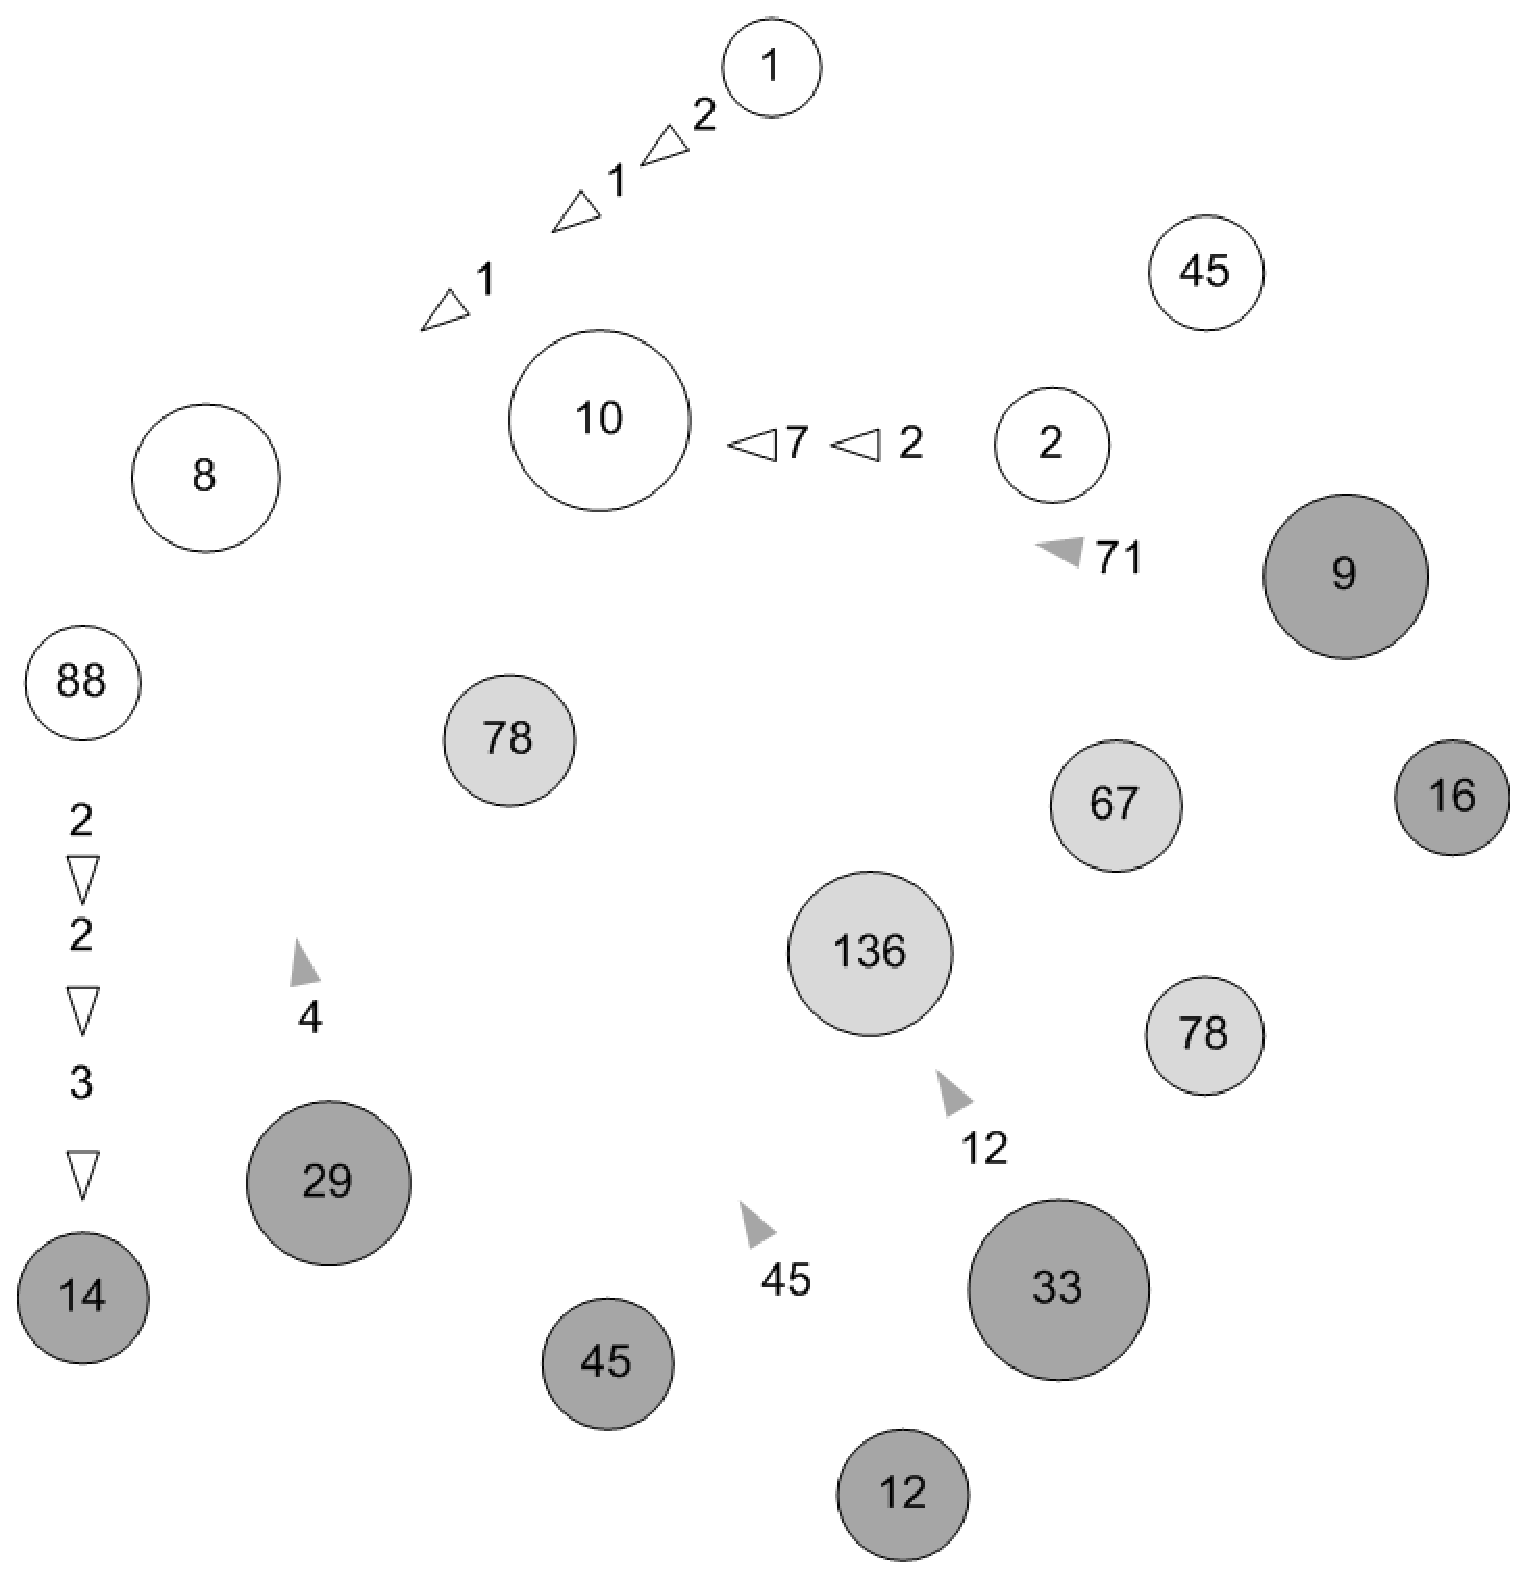
\epsfig{file=./imagenes/naves.eps,width=4cm}
\end{center}
\caption{Simulated screen shot of an early stage of a run in Planet Wars. White planets belong to the player (blue colour in the game), dark grey belong to the opponent (red in the game), and light grey planets belong to no player. The triangles are fleets, and the numbers (in planets and triangles) represent the ships. The planet size means growth rate of the amount of ships in it (the bigger, the higher).}
\label{figura:PlanetWars1}
\end{figure}

A Planet Wars match takes place on a map (see Fig. \ref{figura:PlanetWars1}) that contains several planets (neutral, enemies or owned), each one of them with a number assigned to it that represents the quantity of ships that the planet is currently hosting. 

The aim of the game is to defeat all the ships in the opponent's planets. Although Planet Wars is a RTS game, this implementation has transformed it into a turn-based game, in which each player has a maximum number of turns to accomplish the objective. At the end of the match, the winner is the player that remains alive, or that which owns more ships if more than one survives. 

% Maribel, las comas es que n ingl�s no se usan no? :-)

There are two strong constraints which determine the possible methods to apply to design
a bot: a simulated turn takes \textit{just one second}, and the bot is \textit{not allowed to store any kind of information} about its former actions, about the opponent's actions or about the state of the game (i.e., the game's map).

Therefore, the aim in this paper is to study the improvement of a bot according to the state of the map in each simulated turn (input), returning a set of actions to perform in order to fight the enemy, conquering its resources, and, ultimately, wining the game. In the original game, only two bots are faced but in this paper it is studied what happen when we simulate 4 on 4 battles, i.e., when 4 bots are fighting in the same map.


%%%%%%%%%%%%%%%%%%%%%%%%%%%%%%%%  CO-EVOLUTION  %%%%%%%%%%%%%%%%%%%%%%%%%%%%%%%%
%
\section{Cooperative and Competitive Evolution: Co-Bots}
\label{sec:co-genebot}

%Añadir referencias de Maribel:

There are two types of co-evolution attending to the interaction between the individuals in the population: cooperative and competitive. In this paper, it is described a co-evolutionary algorithm that considers both sides.

Thus, on the one hand, there are 
% Maribel, are will??? eso qu� es " son ser�n" ???--- No uses el futuro, sino el presente o el pasado, no van a luchar, sino que ya han luchado. Lo he cambiado yo
simulated 4 on 4 battles where several bots fight for the same goal: win the battle. That means that every bot competes against each other, or in EA-based concepts, every individual in the population competes for perpetuating its species.
On the other hand, the cooperative factor arises because every 4 on 4 battle is {$all\ versus\ all$}, so a single individual could have assistance 
%cambio la expresi�n tener ayuda
from others for {$killing$} a (temporary) common rival, since at the end, only one must remain (the winner). 

In addition, in the GA the individuals are sharing {$knowledge$}, because they are {$living$} (and fighting) together. If the population is improved, the new offspring {$born$} of the previous parents will behave better.

However, one of the main problems of using EAs for training bots in this problem is 
%Maribel, lo pongo en presente, porque es un problema que existe ahora mismo, no que exist�a.
the huge amount of computational time needed for the evaluation, since it consists in a simulation of several complete battles (in five different and representative maps), moreover a reevaluation process will be performed in every generation (of every individual). The aim of both processes is dealing with the noisy nature of the fitness function due to the pseudo-stochasticity of the problem \cite{Mora_noisy_jcst}.

Theoretically, the use of a co-evolutionary approach would allow 
%Maribel, falta la s
to reduce the number of simulations needed, because the individuals are evaluated in {$groups$}. 

For instance, in a population of 100 individuals, the use of co-evolution considering two individuals per evaluation would reduce the number of evaluations in a half.

In our case, we will test two different approaches, considering both \textit{4 bots simulations} and \textit{2 bots simulations}. The use of two or four individuals of the population in the experiments depends respectively on the use (or not) of previous knowledge. 

%In co-evolution case, for example, if it is used two bots of the population for the co-evolution we only need 50 evaluations. % ya has dicho al principio que es para el caso Co-GA, no hace falta repetir for the Co-GA. 
%Maribel, unas veces dices CGA y otras CoGA o Co-GA, hay que unificarlo
%It is likely that simulations with four bots spent more time that a simulation with two bots, but the question is if the time taken for a  is less that the time taken for two {$2-simulation$}. In that case, the co-evolution decreases the time needed for the training.  % Maribel, aqu� falta una tablita de tiempos o algo que justifique lo que dices.


\subsection{Previous Knowledge vs Auto-generated Knowledge}
\label{sec:knowledge}

In this work we understand as previous knowledge the consideration of a rival evolved in a previous study \cite{Genebot_CEC11}, \textit{ANONYMOUSBot}, which 
proved to be a very competent rival in 1 on 1 battles. This bot will be used as a part of the evaluation process in 4 vs 4 battles.
The aim is to study the influence of this so-called `previous knowledge' in the performance of the proposed Co-Evolutionary Genetic Algorithm (Co-GA). To this end, several experiments have been conducted considering an approach in which two of the rivals are ANONYMOUSBots, and some others in which all the rivals are individuals of the population being evolved.

Thus, two main approaches have been considered:

\begin{itemize}
\item \textbf{Co-evolution with Previous Knowledge}: In this case, battles between two individuals of the population versus two of the best bots (ANONYMOUSBots) have been simulated in the evaluation process. 
It is expected that the Co-Bots are able to learn the basis of the ANONYMOUSBots, and improve for be better rivals in 4 on 4 battles. To this end the algorithm rewards bots that, at least, win in a battle against ANONYMOUSBots. 
Since the approach will evaluate Co-Bots in groups of two, the running time of this approach, will not be reduced in a great factor during the training phase of the bots. 

\item \textbf{Co-evolution with Auto-generated Knowledge}: In this case, battles with four individuals of the population have been tested. 
For this approach the knowledge is included into the individual when it fights in previous battles, i.e., the rivals are included in the learning process. 
In this approach a considerable running time reduction in the comparison with the previous proposal is expected, because the number of evaluations has been reduced to the half.
\end{itemize}

%\subsubsection{}
%\label{sec:knowledge:previous}


%\subsubsection{Co-evolution with Auto-generated Knowledge}
%\label{sec:knowledge:autogenerated}


\subsection{Fitness Functions}
\label{sec:fitness_functions}

In previous works, a bot was evaluated always versus the same bot (a reference bot), several times (in different maps). The fitness function is defined depending of the result of the battle (if the bot wins all its battles or loses in any of them) and the number of turns needed for ending the game. 
For two bots, A and B the fitness was defined as Fig. \ref{fig:fitness_turns_positions}a shows. 

This fitness works well for 1 vs 1 battles, but in this work we have redefined it for 4 vs 4 matches. Moreover two additional evaluation functions have been proposed.

\subsubsection{Fitness based in Position and turns.}
\label{sec:fitness_positions_turns}

This fitness is the natural evolution of the previous one, applied to 4 bots battles. Again, the evaluations are done in several maps. In this case, both the position ($1^{th}$ to $4^{th}$) of the bot in the battle, and the number of turns needed, are included into the formula.

We define the term {$ferocity$}, regarding a bot that wins all its battles. This factor is included in the fitness computation as the sum of turns the bot has needed to win. This sum is considered to select the best bot when more than one wins all its battles, since a bot that wins in less turns is better than other that wins needing more. 
In some other cases, the sum of turns is called {$sturdy$}, and opposite to the {$ferocity$}, it is desirable a bot that take more turns in being defeated. In Fig. \ref{fig:fitness_turns_positions}b there is a formal definition of this fitness.

\begin{figure}[h]
\tiny
\begin{subfigure}[!]{0.52\textwidth}
\begin{algorithmic}
        \State{$A,B\in Population $}
        \If {A WINs always}
            \If{B LOSEs some battle}
                \State A is better than B
            \ElsIf{A take less turns than B}
                \State A is better than B
            \Else
                \State B is better than A
            \EndIf
        \Else
             \If{B WINs always}
                \State B is better than A
            \ElsIf{A take less turns than B}
                \State B is better than A
            \Else
                \State A is better than B
            \EndIf
        \EndIf
        \end{algorithmic}
        \caption{Fitness considered in 1 vs 1 battles}
        \label{fig:fitness_turns_positions:2}
\end{subfigure}
\begin{subfigure}[!]{0.52\textwidth}
    \begin{algorithmic}
        \State{$A,B\in Population $}
        \If {A average position $<$ B average position}
            \State A is better than B
        \ElsIf{A average position $>$ B average position}
            \State B is better than A
        \Else
            \If{A,B is always $1^{th}$}
                \If{A take less turns than B}
                    \State A is better than B
                \Else
                    \State B is better than A
                \EndIf
            \Else
                \If{A take less turns than B}
                    \State B is better than A
                \Else
                    \State A is better than B
                \EndIf
            \EndIf
        \EndIf
    \end{algorithmic}
    \label{fig:fitness_turns_positions:co}
\caption{Fitness considered in 4 vs 4 battles}
\end{subfigure}
\caption{Fitness functions based in turns and positions}
\label{fig:fitness_turns_positions}
\end{figure}

In this fitness, we are only interested in the final result (position and number of turns). We do not include in the analysis how the bot has reached them. The problem of this function is that the consideration of two different terms makes it difficult the comparison between different evaluations. In order to let easier comparisons two other fitness functions have been defined. 

Both of them are based in the percentage of ships belonging to each player in every turn. They are normalized considering the total number of ships in the game for that turn (including neutrals ships in neutral planets). For each player, we have a different {$cloud$} of ships.

%as Fig.\ref{figura:nubecita} shows. 
%\begin{figure}[h]
%\begin{center}
%  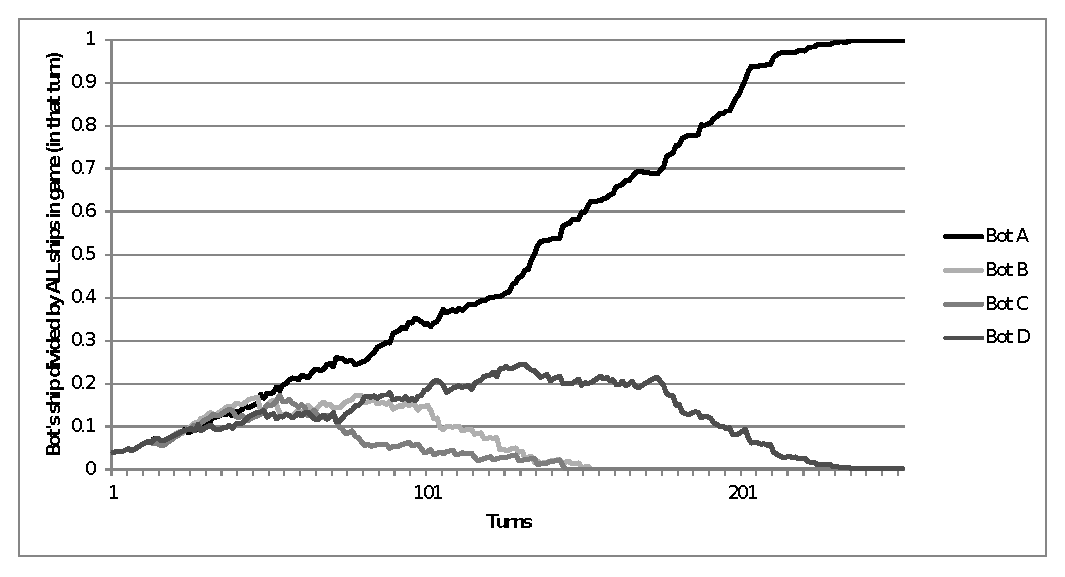
\epsfig{file=imagenes/nubecita.eps,width=4cm}
%\end{center}
%\caption{Representation of the number of ships of each bot in each turn} 
%\label{figura:nubecita}
%\end{figure}

Below, are described the two alternatives to deal with this cloud of points for the fitness function: the use of slopes and areas.


\subsubsection{Fitness based in Slope.}
\label{sec:fitness_slope}

For this fitness, a square regression analysis is computed in order to transform the cloud of points into a simple line. The line is represented as {$y = \alpha \times x + \beta $}, where {$\alpha$} and {$\beta$} are calculated as shown in Equations \ref{eq:alpha} and \ref{eq:beta}, computing a least squares regression. For every bot in the simulation we calculate $\alpha$ and ($slope$). This $slope$ is the fitness of every bot for that simulation. A graphical example can be seen in Fig. \ref{figura:nubecita:pendiente}.

\begin{equation}
\label{eq:alpha}
        \alpha = \frac{\sum_{i=1}^{n}(X_{i} - \bar{X_{i}})(Y_{i} - \bar{Y_{i}})}{\sum_{i=1}^{n}(X_{i} - \bar{X_{i}})^{2}}
\end{equation}

\begin{equation}
\label{eq:beta}
        \beta = \bar{Y}-\alpha\bar{X}
\end{equation}


\begin{figure}[h]
\centering
%\hspace*{-1in}
  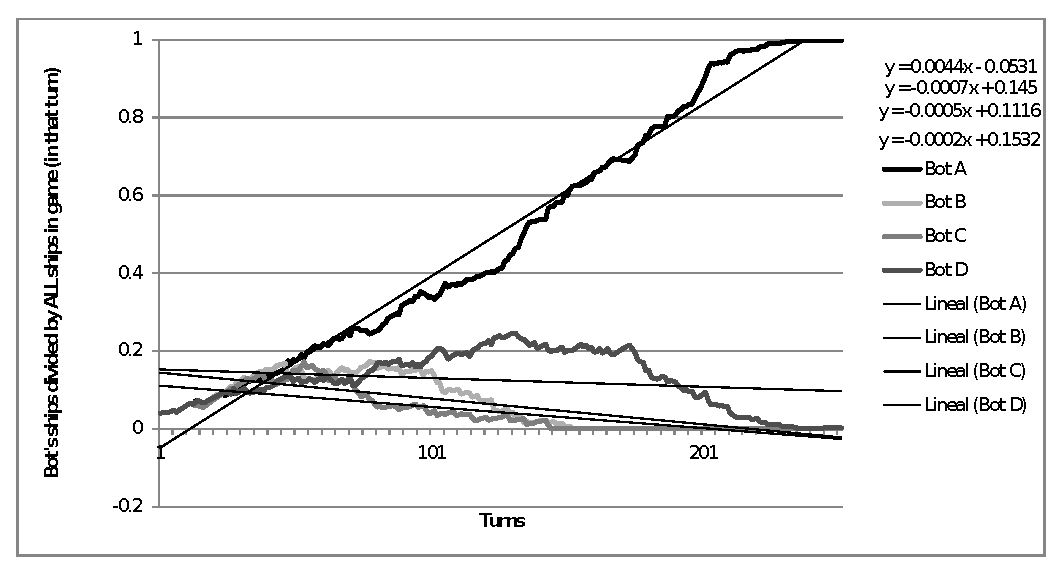
\epsfig{file=imagenes/nubecita_pendiente.eps,width=0.8\textwidth}
\caption{Fitness based in Slope: number of ships of every bot in each turn}
\label{figura:nubecita:pendiente}
\end{figure}


%\begin{figure}[h]
%\centering
%\hspace*{-1in}
%\begin{subfigure}[H]{0.4\textwidth}
%	\large
%    \begin{equation}
%        \alpha = \frac{\sum_{i=1}^{n}(X_{i} - \bar{X_{i}})(Y_{i} - \bar{Y_{i}})}{\sum_{i=1}^{n}(X_{i} - \bar{X_{i}})^{2}}
%    \end{equation}
%    \begin{equation}
%        \beta = \bar{Y}-\alpha\bar{X}
%    \end{equation}
%    \caption{Least Squares Regression}
%    \label{equation:LeastSquares}
%\end{subfigure}
%\hfill
%\hspace*{0.2in}
%\begin{subfigure}[H]{0.7\textwidth}
%\begin{center}
%  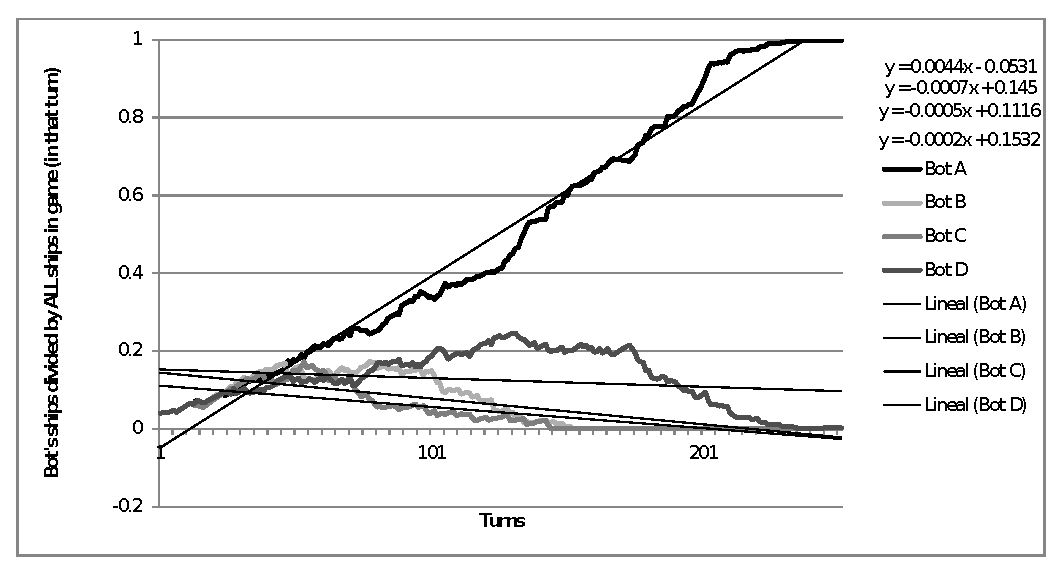
\epsfig{file=imagenes/nubecita_pendiente.eps,width=1.1\textwidth}
%\end{center}
%\caption{Number of ships of every bot in each turn} %Maribel, cambio if por of
%\label{figura:nubecita:pendiente}
%\end{subfigure}
%\caption{Fitness based in Slope}
%\end{figure}

Theoretical maximum and minimum values are set for this fitness. An optimum bot that wins in the first turn, has an ideal slope of {$1$}, so this is the maximum value of our fitness. On the other hand, a bot that loses in the first turn,  has a slope of {$-1$}. Thus, if we calculate the $slope$, we know if the bot {$WINs$} ({$slope>0$}) or {$LOSEs$} {$slope<0$}. 
The values of the different battles are summed to compute the global $slope$. Then, the bot with the highest value will be the best is each turn or battle. 

%Several evaluations in different maps was using, so it's need operate with fitness. In that case, only sum the slope of all the evaluations of the bot. Maribel, esto ya lo has dicho antes y adem�s l�a m�s la cosa as� que lo he eliminado. Adem�s expresiones como "was using" est�n mal, qu� quieres decir? fue usando? eso en ingl�s no se dice.

\subsection{Fitness based in Area.}
\label{sec:fitness}

In this case, the integral of the curve of the bot's live-line is used for calculating the area that is `covered' by the fitness cloud of points (see Equation \ref{eq:area}). This {$area$} is normalized considering the number of turns, and thus it represents the average percentage of ships during the battle for each player. 
%An example is shown in Fig. \ref{figura:nubecita:area}.

\begin{equation}
        area=\frac{\int_{0}^{t}\%ships(x)dx}{t}
    \label{eq:area}
\end{equation}

% \begin{figure}[h]
% \begin{center}
%   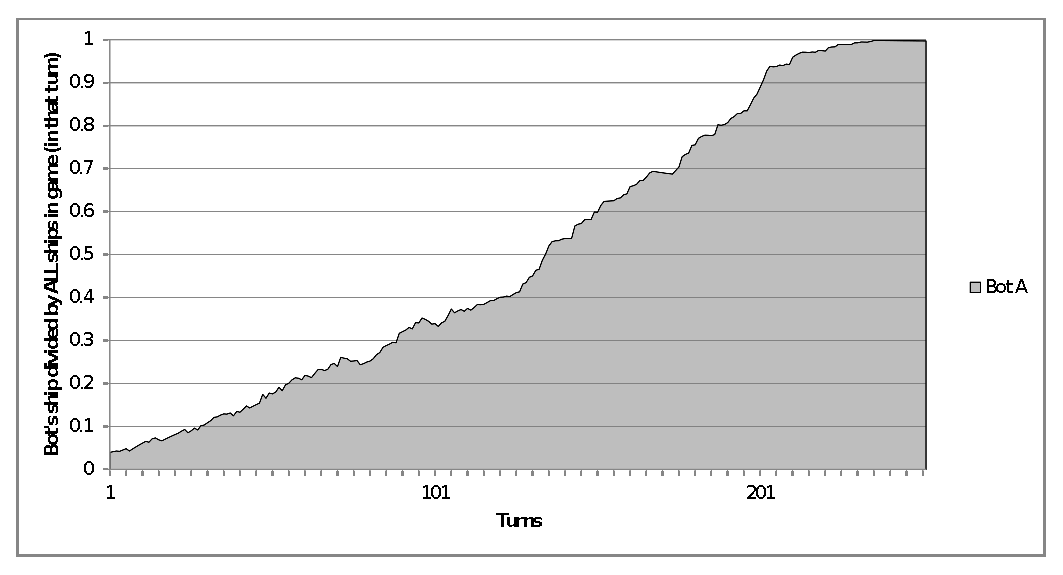
\epsfig{file=imagenes/nubecita_integral.eps,width=0.7\textwidth}
% \end{center}
% \caption{Fitness based in Area. Example of area under the live-line curve.}
% \label{figura:nubecita:area}
% \end{figure}

%\begin{figure}[h]
%\centering
%\hspace*{-1in}
%\begin{subfigure}[H]{0.4\textwidth}
%	\large
%    \begin{equation}
%        area=\frac{\int_{0}^{t}\%ships(x)dx}{t}
%    \end{equation}
%    \caption{Calculus of the area}
%    \label{equation:area}
%\end{subfigure}
%\begin{subfigure}[H]{0.6\textwidth}
%\begin{center}
%  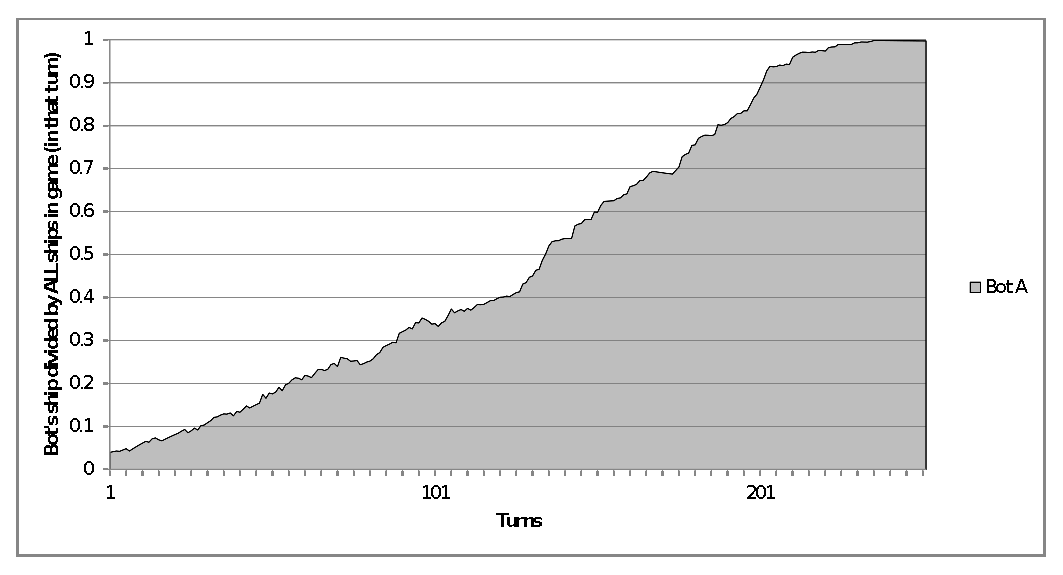
\epsfig{file=imagenes/nubecita_integral.eps,width=0.6\textwidth}
%\end{center}
%\caption{Example of area under the live-line curve.} 
%\label{figura:nubecita:area}
%\end{subfigure}
%\caption{Fitness based in Area}
%\end{figure}

As in previous case, maximum and minimum values has been set for this fitness. If an optimal bot wins in the first turn, the area of each live-line is close to {$1$}, so this is the maximum value of the fitness. Otherwise, if a bot loses in the first turn, its live-line area is close to {$0$}. In this case, we do not extract additional information related with which bot wins the battle, because the area of the live-line is not related with the winner of the battle. Thus, we are losing some information.

%%%%%%%%%%%%%%%%%%%%%%%%%%%%%%%   EXPERIMENTS  %%%%%%%%%%%%%%%%%%%%%%%%%%%%%%%%
%
\section{Experiments and Results}
\label{sec:experiments}

Several experiments have been conducted in order to study different issues of the proposed approaches, but having in mind that the main objective is the improvement of bots using a co-evolutionary algorithm. The set of parameters considered in the Co-GA is shown in Table \ref{tabla:GA}. 
For each one of the presented approaches (combinations of fitness functions and knowledge-related methods), ten executions of the Co-GA have been performed.

\begin{table}
\centering
\begin{tabular}{|c | c | c | c | c | c |}
\hline
Population Size & Generations & Crossover prob. & Mutation prob. & Elitism & Tournament size \\
\hline
100 & 200 & 0.6 & 0.1 & 20 & 2 \\
\hline
\end{tabular}
\caption{Table with the parameters used in the Co-GA.}
\label{tabla:GA}
\end{table}

As a first set of results, the average time consumed in the run of every generation is plotted in Fig. \ref{figura:tiempos}. The values are, as expected, reduced in a half in the previous knowledge approach (2 individuals per evaluation), and in 3/4 in the auto-generated knowledge (4 individuals per evaluation). This could be non-surprising results, but there should be considered than the original method evaluated 1 vs 1 battles, which are usually finished in less time than 4 vs 4 matches.

%In addition, the time used for the evaluation in each generation was measure to compare the time needed for the GA. As you can see in Fig.the co-evolution is faster than a simple GA, decreasing the time near to the half in the case of the previously-knowledge fitness, and a quarter in the autogenerated-knowledge fitness. 

\begin{figure}[h!t]
\tiny
\begin{center}
  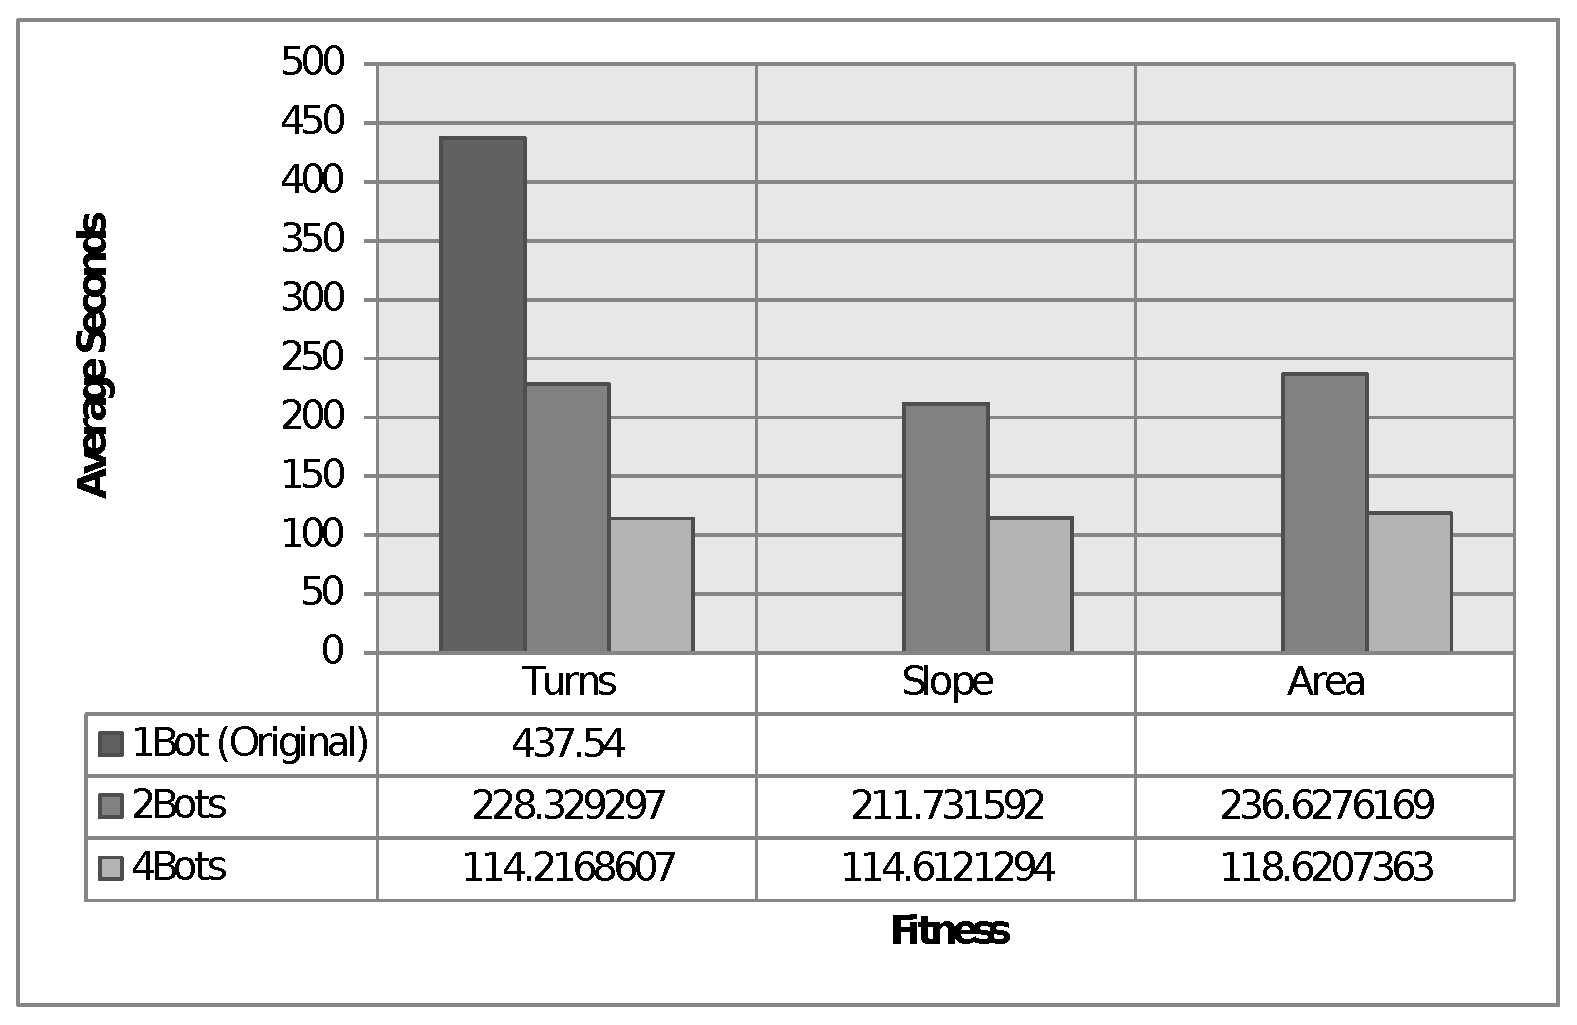
\epsfig{file=./imagenes/tiempos_segundos.eps,width=6cm}
\end{center}
\caption{Average time per generation (secs)}
\label{figura:tiempos}
\end{figure}

The second analysis concerns the fitness evolution. To this end the best, worst, median and average (with standard deviation) fitness values are studied.
In Fig. \ref{estudio:fitness} it can be seen the corresponding values to the best execution in every case, i.e. that of the 10 runs which obtained the considered as the best bot.

In auto-generated knowledge fitness (Fig.\ref{estudio:fitness:auto}) it can be observed an homogeneous distribution throughout the generations, because the individuals are learning all of all, so the differences among them remain equal (in some limits) along the whole evolutionary process. That figure shows a high variability (or oscillations) in the best fitness graph, due to the rivals (in evaluation) are included in the learning process, so the population is not adapted to a common behavioural pattern, but every individual must learn to compete against (potentially) N-1 different bots. This means that the best individual varies frequently.

In the case of previously knowledge fitness (Fig.\ref{estudio:fitness:previous}), it can be noticed a slight improvement, on the average fitness in the first generations. This happens because more and more individuals are able to beat the bots considered as rivals (ANONYMOUSBots), an expected result. In addition, and due to this behavioural pattern to fight with, the evolution of the best fitness presents less variations along the generations.

Anyway, the noisy nature of the fitness function due to the problem itself \cite{Mora_noisy_jcst}, remains here and this means that traditional evolution graphs (clear fitness improvement with very slight variations along generations) could not be obtained.

\begin{figure}[h!]
    \centering
    \begin{subfigure}[H]{0.49\textwidth}
        \begin{center}
            \epsfig{file=imagenes/2G-turnos_all.eps,width=1\textwidth, trim = 10mm 40mm 10mm 40mm, clip}
            \epsfig{file=imagenes/2G-pendiente_all.eps,width=1\textwidth, trim = 10mm 40mm 10mm 40mm, clip}
            \epsfig{file=imagenes/2G-area_all.eps,width=1\textwidth, trim = 10mm 40mm 10mm 40mm, clip}
        \end{center}
        \caption{Methods with previous knowledge: from top to down Turns/Position, Slope and Area}
        \label{estudio:fitness:previous}
    \end{subfigure}
    \begin{subfigure}[H]{0.49\textwidth}
        \begin{center}
            \epsfig{file=imagenes/4G-turnos_all.eps,width=1\textwidth, trim = 10mm 40mm 10mm 40mm, clip}
            \epsfig{file=imagenes/4G-pendiente_all.eps,width=1\textwidth, trim = 10mm 40mm 10mm 40mm, clip}
            \epsfig{file=imagenes/4G-area_all.eps,width=1\textwidth, trim = 10mm 40mm 10mm 40mm, clip}
        \end{center}
        \caption{Methods with auto-generated knowledge: from top to down Turns/Position, Slope and Area}
        \label{estudio:fitness:auto}
    \end{subfigure}
    \caption{Best, worst, average, median and Std.Dev for fitness in every generation.}
    \label{estudio:fitness}
\end{figure}

Next a comparison between the methods has been performed. However, since the fitness computation function is different for each method, they can not be directly compared (as they have different magnitudes). So it is necessary to perform simulations in a wide range of maps and enemies to study how good they are.

First a fool bot (GoogleBot) has been chosen to simulate 400 battles. In these battles, every bot obtained by Co-GA has to fight against 3 of these bots. The results have been excellent, with 100\% of victories of the Co-Bots against them.

Then, a tough set of rivals has been considered, being three copies of the best bot previously obtained in other work, namely three ANONYMOUSBots. 500 battles against them have been simulated, and the results are shown in Fig.\ref{figura:supertest}. The best average results are obtained for the Co-Bots obtained using previous knowledge, since they were trained to deal with at least two of them during the evolution. However, the scenario here is quite different since there is another ANONYMOUSBot as rival. As a general result, in both cases, the worst performance is achieved considering turns/position based fitness.

%\begin{figure}[H]
%\tiny
%\begin{center}
%  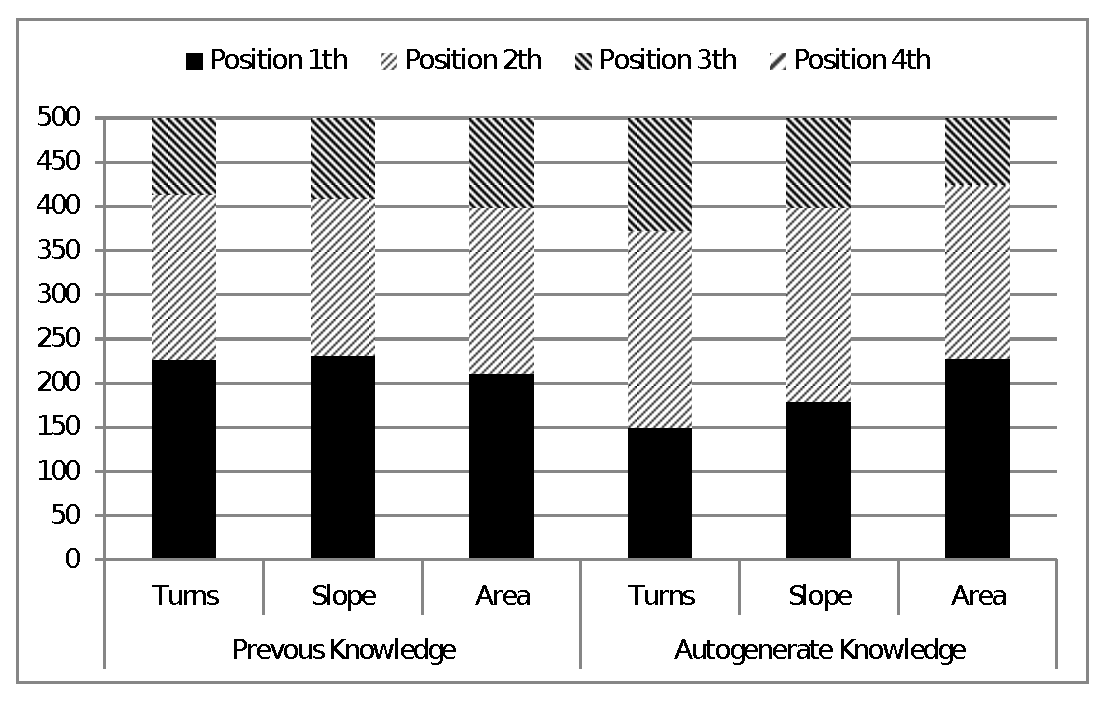
\epsfig{file=imagenes/contra_2_genebots+1google_grafica.eps,width=7cm}
%\end{center}
%\caption{Generation average time of execution to each fitness and knowledge method}
%\label{figura:tiempos}
%\end{figure}

\begin{figure}[h!]
\tiny
\begin{center}
  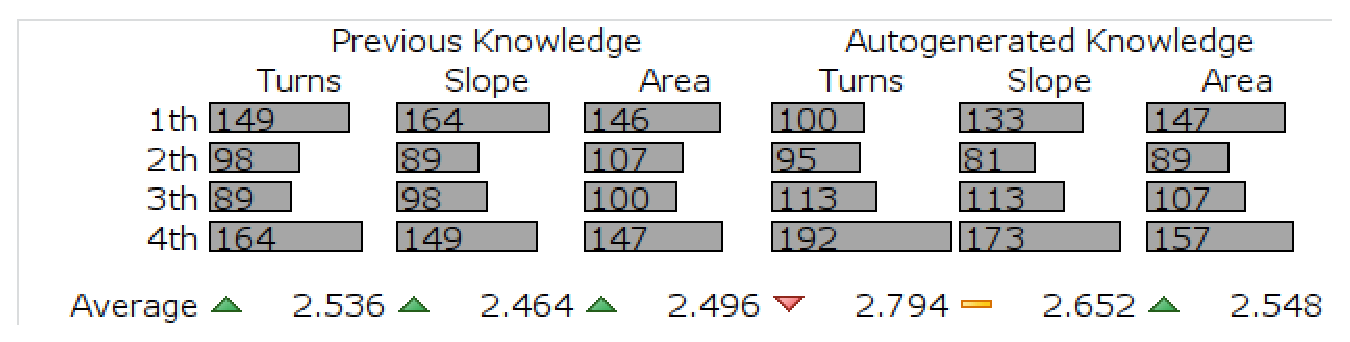
\epsfig{file=imagenes/super_tabla.eps,width=0.7\textwidth}
  %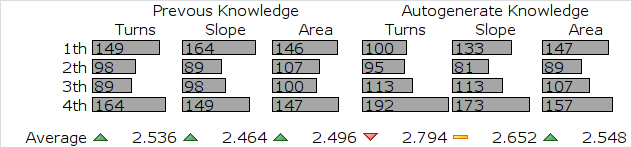
\includegraphics[width=0.7\textwidth]{"imagenes/super_tabla.eps"}
  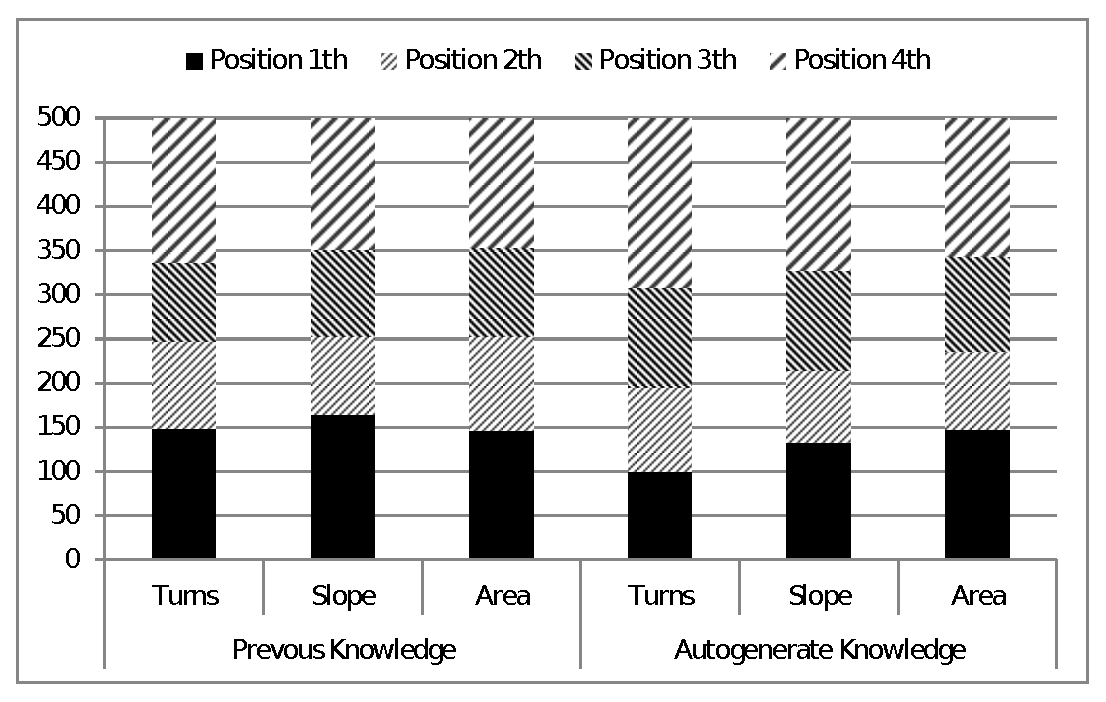
\epsfig{file=imagenes/contra_3_genebots_grafica.eps,width=7cm}
\end{center}
\caption{Results (positions) of 500 4 vs 4 battles between 3 ANONYMOUSBots and a bot per each method.}
\label{figura:supertest}
\end{figure}
 
To study whether the bots actually achieved by the turn-based fitness are really less competitive, we have conducted a simulation (3 vs 3) matching the three bots achieved by the three fitness methods using, separately per knowledge approach. Fig.\ref{figure:comparativa:fitness:separados} shows the results for each knowledge method. It is complemented with the summed results plotted in Fig.\ref{figure:comparativa:fitness:total}, which shows the sum per fitness method (for the two knowledge approaches).
As it can be seen the bots obtained with the fitness based in turns/positions perform clearly worse than the others.

\begin{figure}[h!]
    \advance\leftskip-2.5cm
    \begin{subfigure}[H]{0.7\textwidth}
        \begin{center}
            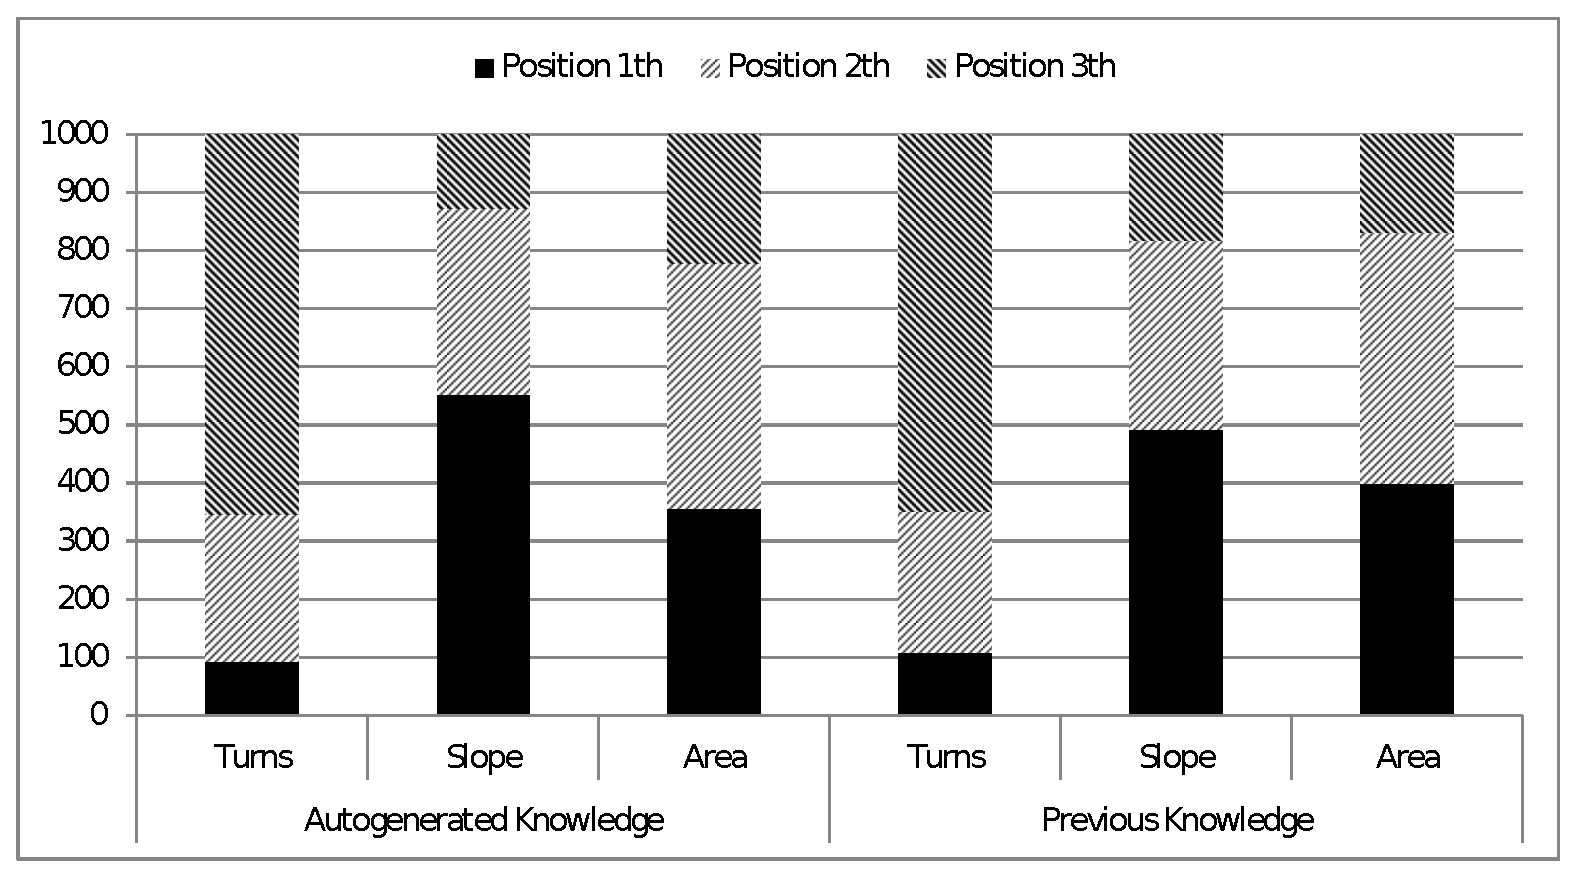
\epsfig{file=imagenes/comparativa_fitness_separados.eps,width=1\textwidth}
        \end{center}
        \caption{Results (positions) per knowledge approach}
        \label{figure:comparativa:fitness:separados}
    \end{subfigure}
    \begin{subfigure}[H]{0.7\textwidth}
        \begin{center}
            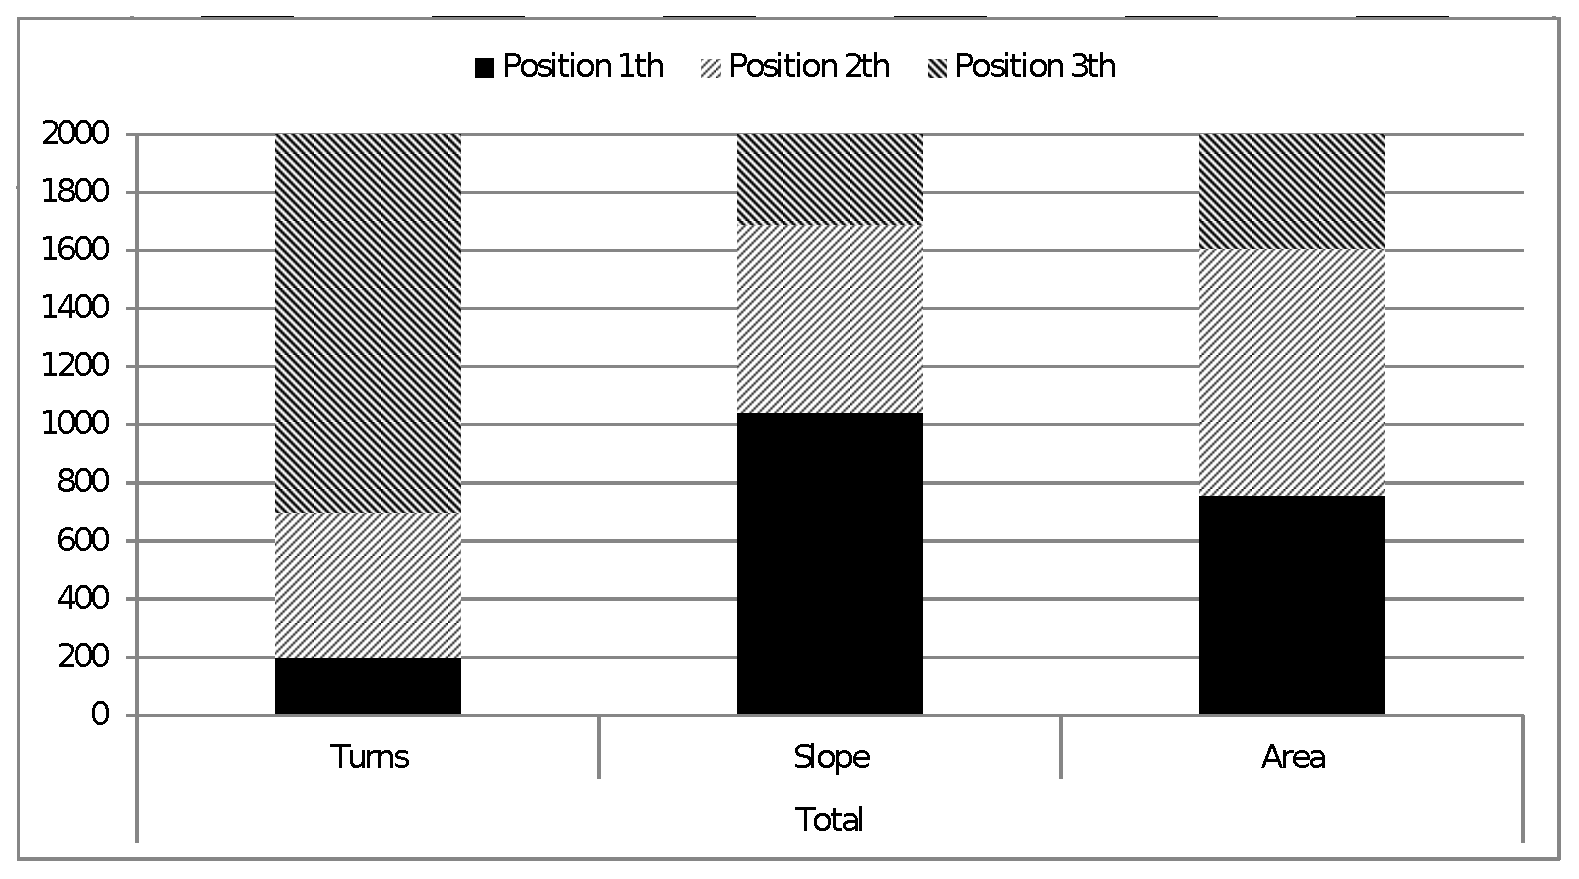
\epsfig{file=imagenes/comparativa_fitness_total.eps,width=1\textwidth}
        \end{center}
        \caption{Total sum of results (same positions) per fitness method, considering both knowledge approches}
        \label{figure:comparativa:fitness:total}
    \end{subfigure}
    \caption{Results of 1000 3 vs 3 battles between the obtained bots.}
    \label{figure:comparativa:fitness}
\end{figure}

Finally, the top four of the yielded bots are tested in 500 battles between them. There is one bot per fitness function, without considering the turn-based ones (since they are worse).  Fig.\ref{figura:todos_contra_todos} shows how the bots have performed and their position in the battles. As it can be seen Slope-based Co-Bots are better than Area-based ones. Similarly, bots trained with previous knowledge, perform better than those with auto-generated knowledge.

\begin{figure}[h!]
\tiny
\begin{center}
  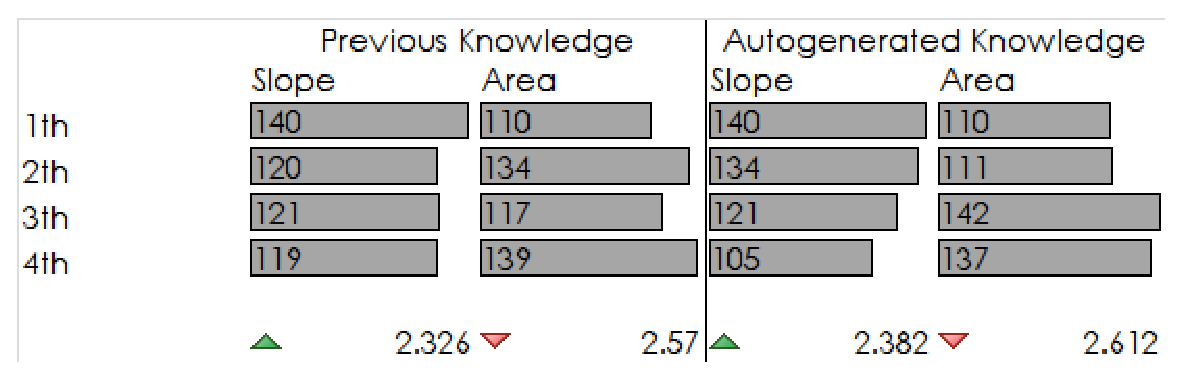
\epsfig{file=imagenes/todos_contra_todos.eps,width=0.85\textwidth, trim = 1mm 0mm 0mm 1mm, clip}
  %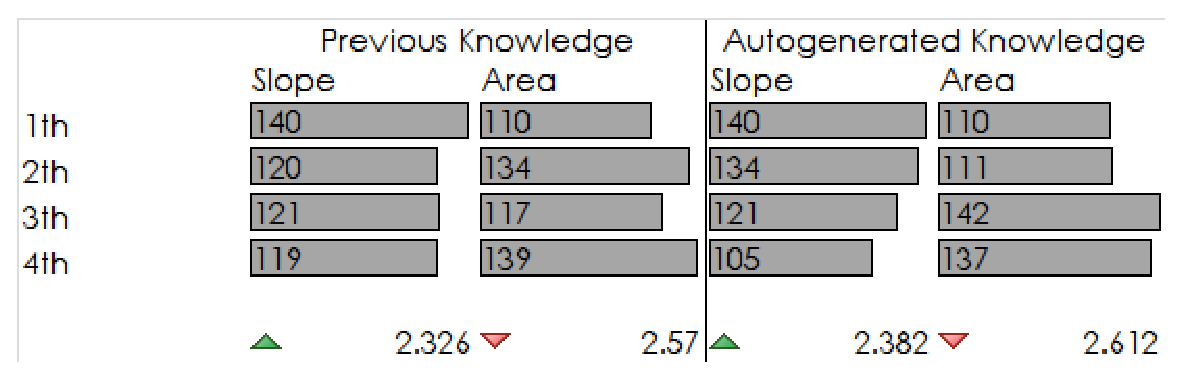
\includegraphics[width=0.85\textwidth, trim = 1mm 0mm 0mm 1mm, clip]{"imagenes/todos_contra_todos.eps"}
\end{center}
\caption{Results (positions) of 500 4 vs 4 battles matching the four best bots obtained (one per approach).}
\label{figura:todos_contra_todos}
\end{figure}



%%%%%%%%%%%%%%%%%%%%%%%%%%%%%%  CONCLUSIONS  %%%%%%%%%%%%%%%%%%%%%%%%%%%%%%%
%
\section{Conclusions and Future Work}
\label{sec:conclusions}

This paper presents some cooperative co-evolutionary approaches for improving autonomous agents for playing the RTS game Planet Wars. They are trained for 4 on 4 battles, considering two types of evaluation: based in previous knowledge (i.e. against a previously obtained bot), and with auto-generated knowledge (i.e. the rivals are included in the learning process). In addition three different fitness functions have been tested for each method: a position/turns based one, linear regression model and area computation, regarding the number of ships belonging to the bot/individual to be evaluated in the last cases.

The first remarkable result is the significant reduction of the training time needed, due to the use of co-evolution.

It has been shown that a position/turn-based fitness function is less effective for training than one based on the study of curve resources (ships in this paper), in co-evolutionary approaches. Regarding the two mathematical fitness, the one based on the slope has proven to be slightly better, possibly due to a better representation of the bots victories against losses.
Another interesting result point to that the use of previous knowledge can make a difference, but not very significant. 
In the future it may be interesting to go deep in the study on the real influence of the previous knowledge.

Moreover this paper opens up new lines of research on the proposed problem. Such as the study of different ways for extracting knowledge from the population for co-evolution, for example the use of a Hall of Fame as proposed by the authors in \cite{Nogueira_HoF2013}, %(evaluar contra los X mejores individuos)
or the study of other mathematical fitness approximations.
Regarding the co-evolution, it could be studied a competitive approach in which there could be different subpopulations devoted to improve different controllers for agents.

%Finally, it would be interesting to study if at CO-GA algorithm as the one discussed in this paper needs a fitness function. Opting instead to use the co-evolution to solve the crossover and propagation.

%%%%%%%%%%%%%%%%%%%%%%%%%%%%%%   ACKNOWLEDGEMENTS %%%%%%%%%%%%%%%%%%%%%%%%%%%%%%
%
%\section*{Acknowledgements}

%This paper has been funded in part by projects P08-TIC-03903 (Andalusian Regional Government), TIN2011-28627-C04-02 (Spanish Ministry of Science and Innovation), and project 83 (CANUBE) awarded by the CEI-BioTIC UGR.

\bibliographystyle{splncs}
\bibliography{genebot}


\end{document}
